% !TEX root = /home/fred-olav/afgv/src/preamble.tex
\input preamble.tex
\huge
\centerline{\bf Heldagsprøve Fabrikkautomasjon 23/24}  \bigskip
\normalsize
\vskip 1cm 
Kompetansemål:
Prøven dekker alle kompetansemål i automatiseirngsfaget fra VG1 til VG3 auto, men hanlder spesielt om:
\begin{itemize}[noitemsep]

\item montere og sette i drift sikkerhetskomponenter og -utstyr for nødstopp- og sikkerhetskretser, og gjøre rede for sikkerhetskategoriene Safety Integrity Level (SIL) og Performance Level (PL)
\item programmere, montere og sette i drift programmerbare styresystemer for elektriske-, pneumatiske- og hydrauliske anlegg og gjøre rede for hvordan utstyret fungerer, og hvilke funksjoner det har
\item simulere, sette i drift, programmere og optimalisere robot og gjøre rede for roboters funksjon og anvendelse i automatiserte anlegg
\end{itemize}

Alle ark som leveres inn skal ha elevens navn. \\ 

\oppgave{}%7
Du får i oppdrag å programmere og testkjøre sekvensen for transport av kumlokk på transportbåndene inkludert overføring og mottak til roboten. (ikke sekvensen i roboten). Sekvensen starter når det kommer et kumlokk inn på transportbåndet og avsluttes når det er ferdig maskinert og kommet til andre enden. Bruk tydelige navn på variabeler for å beskrive hvilke sensorer som starter du ulike trinnene. 
\vskip 1cm
• Planlegg, beskriv gjennomføring og dokumenter jobben. Lag skisser til forklaringene. 
\vskip 1cm
\oppgave{}%7
 Du får i oppdrag å legget til et bilde på PLS-ens HMI. Det er et ønske at transportbåndenes hastighet skal vises i displayet og at hastigheten skal kunne justeres fra HMI bildet  

\vskip 1cm
• Lag et blokkskjema over løsningen og nødvendig PLS program.
$$\includegraphics[width=15.5cm]{./aFab2324x2-1.eps}$$
$$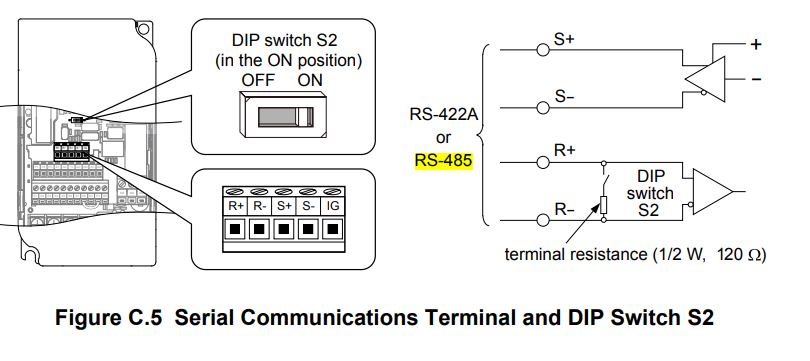
\includegraphics[width=15.5cm]{./aFab2324x2-1-2.png}$$
$$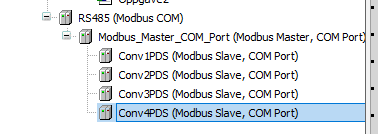
\includegraphics[width=15.5cm]{./aFab2324x2-2.png}$$
$$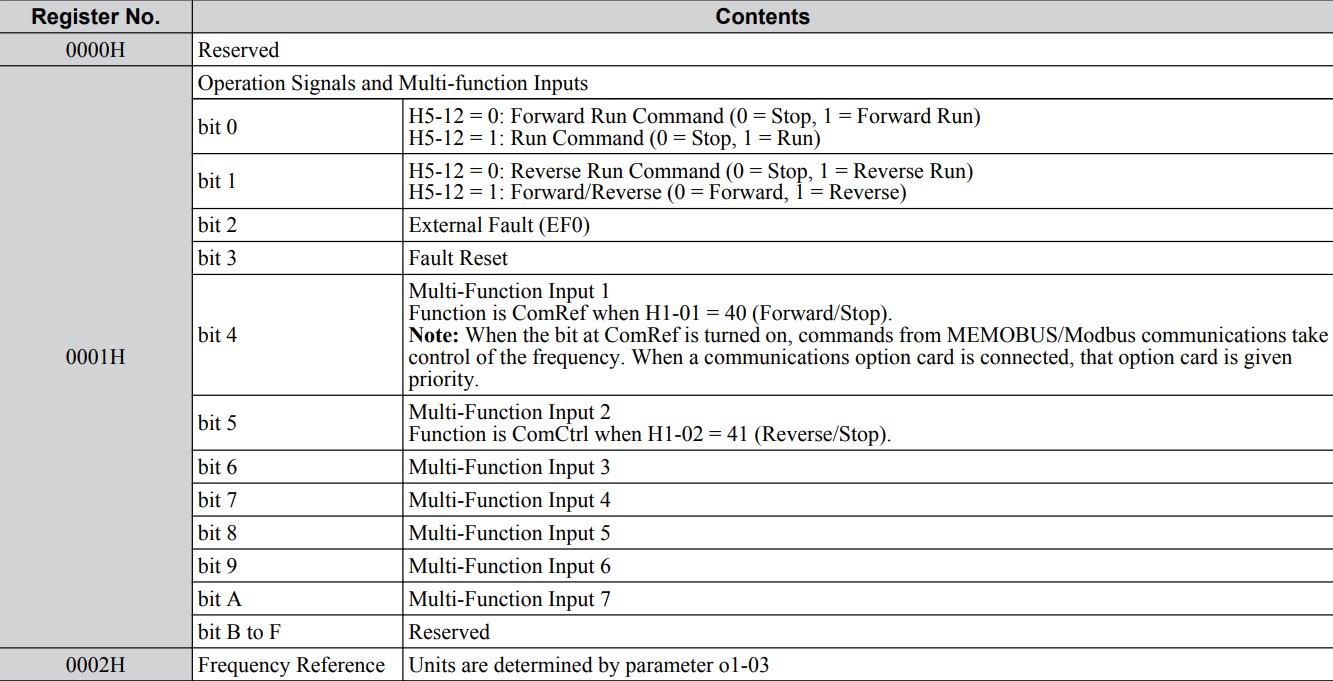
\includegraphics[width=15.5cm]{./aFab2324x2-1-1.png}$$
$$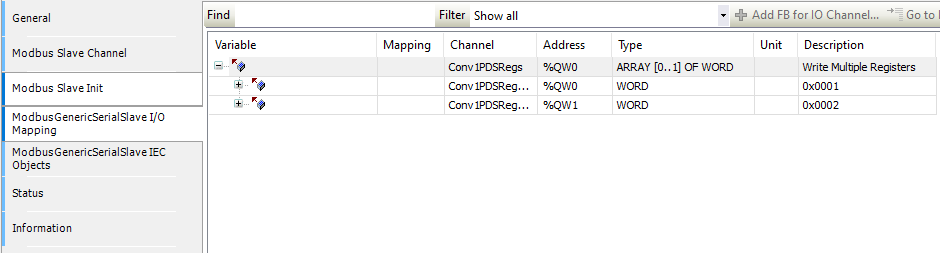
\includegraphics[width=15.5cm]{./aFab2324x2-3.png}$$
$$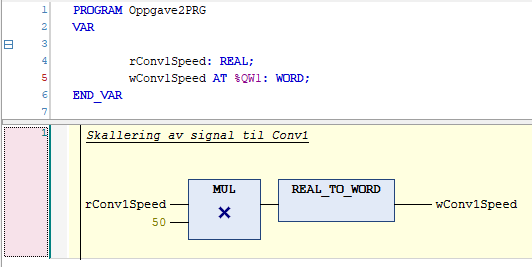
\includegraphics[width=15.5cm]{./aFab2324x2-4.png}$$
$$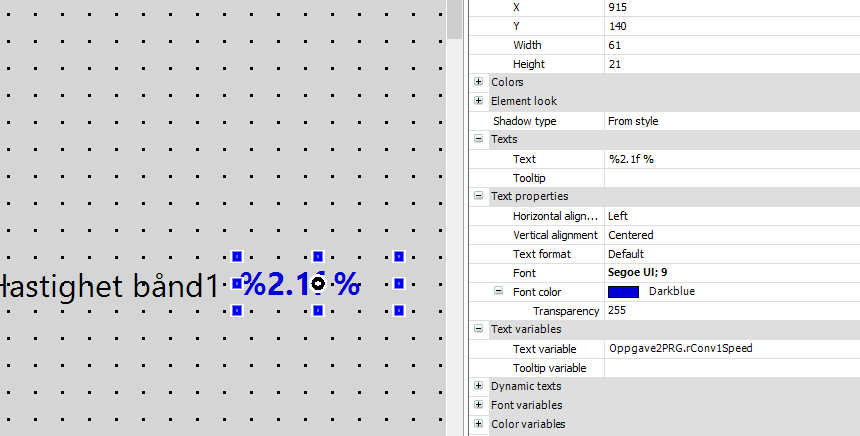
\includegraphics[width=15.5cm]{./aFab2324x2-5.png}$$
$$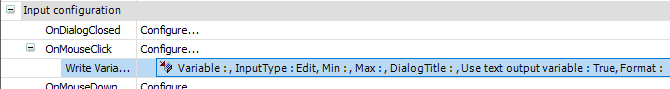
\includegraphics[width=15.5cm]{./aFab2324x2-6.png}$$
$$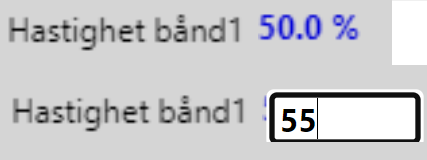
\includegraphics[width=15.5cm]{./aFab2324x2-7.png}$$

\vskip 1cm
\oppgave{}%7
Sjefen er veldig bestemt på at "anlegget” skal ha sikkerhetsnivå PL e, men lurer på om dette er mulig. Du har fått i oppdrag å koble opp og teste sikkerhetsfunksjonen rundt nødstopp av transportbåndene.
\vskip 1cm
• Planlegg, beskriv gjennomføring og dokumenter jobben. Lag skisser til forklaringene. 
\vskip 1cm
$$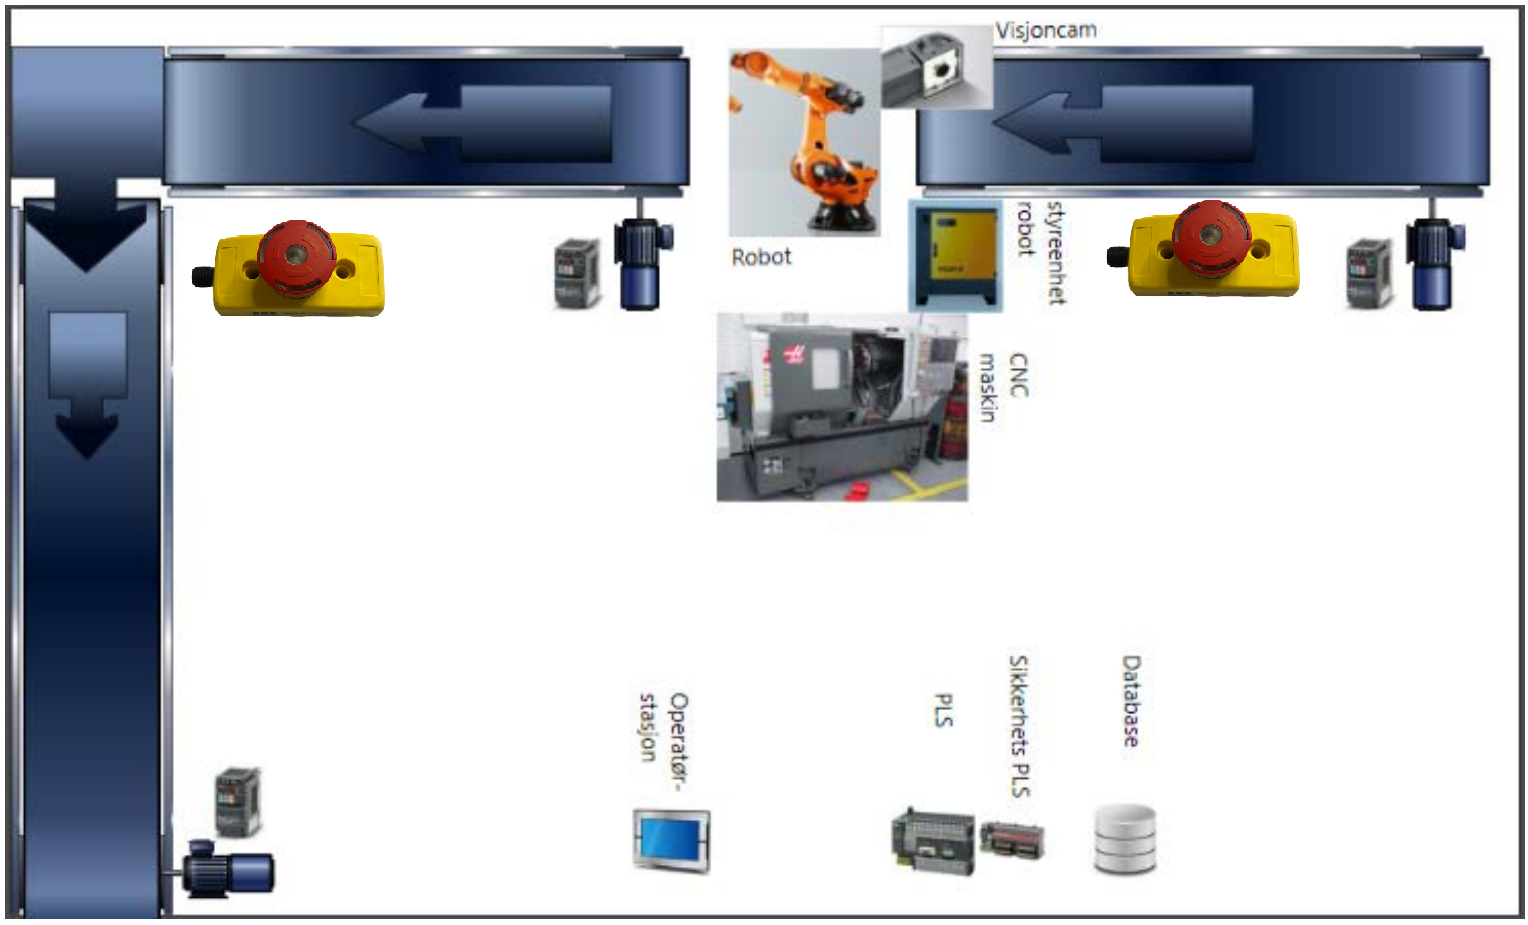
\includegraphics[width=15.5cm]{./aFab2324x3-5.png}$$
$$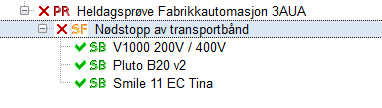
\includegraphics[width=15.5cm]{./aFab2324x3-1.png}$$
$$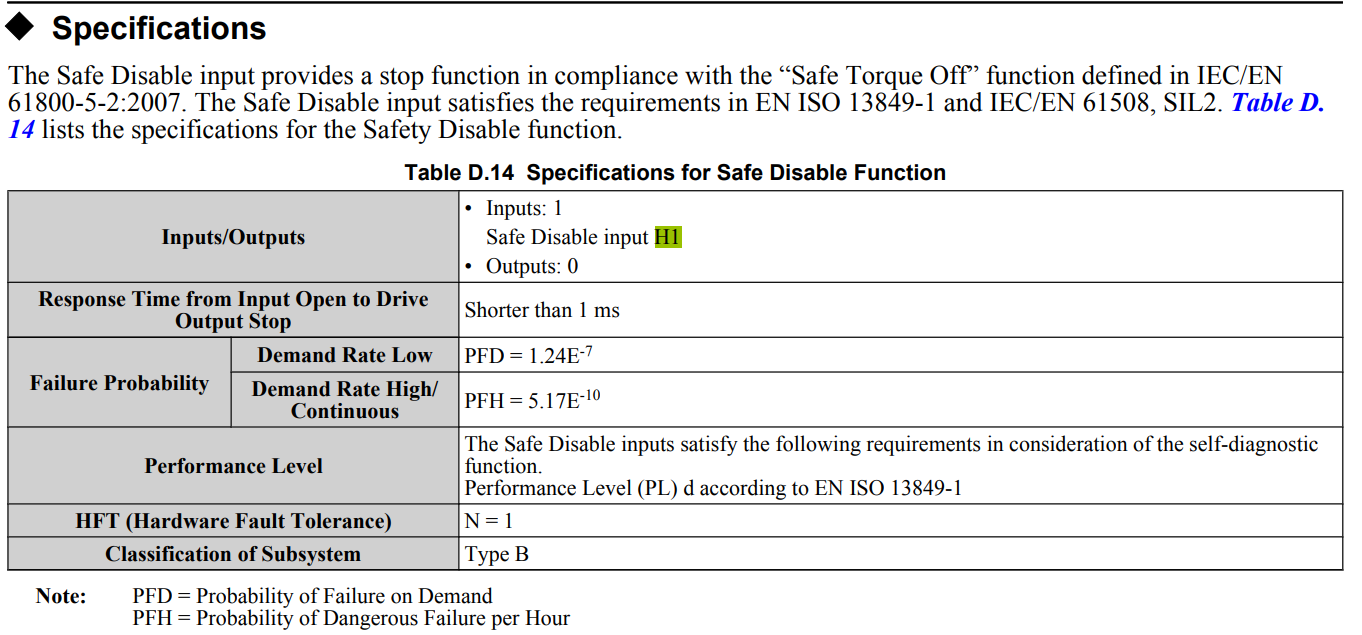
\includegraphics[width=15.5cm]{./aFab2324x3-2.png}$$
$$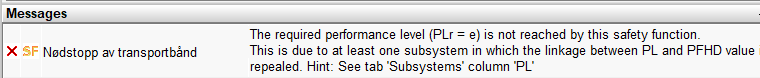
\includegraphics[width=15.5cm]{./aFab2324x3-3.png}$$
$$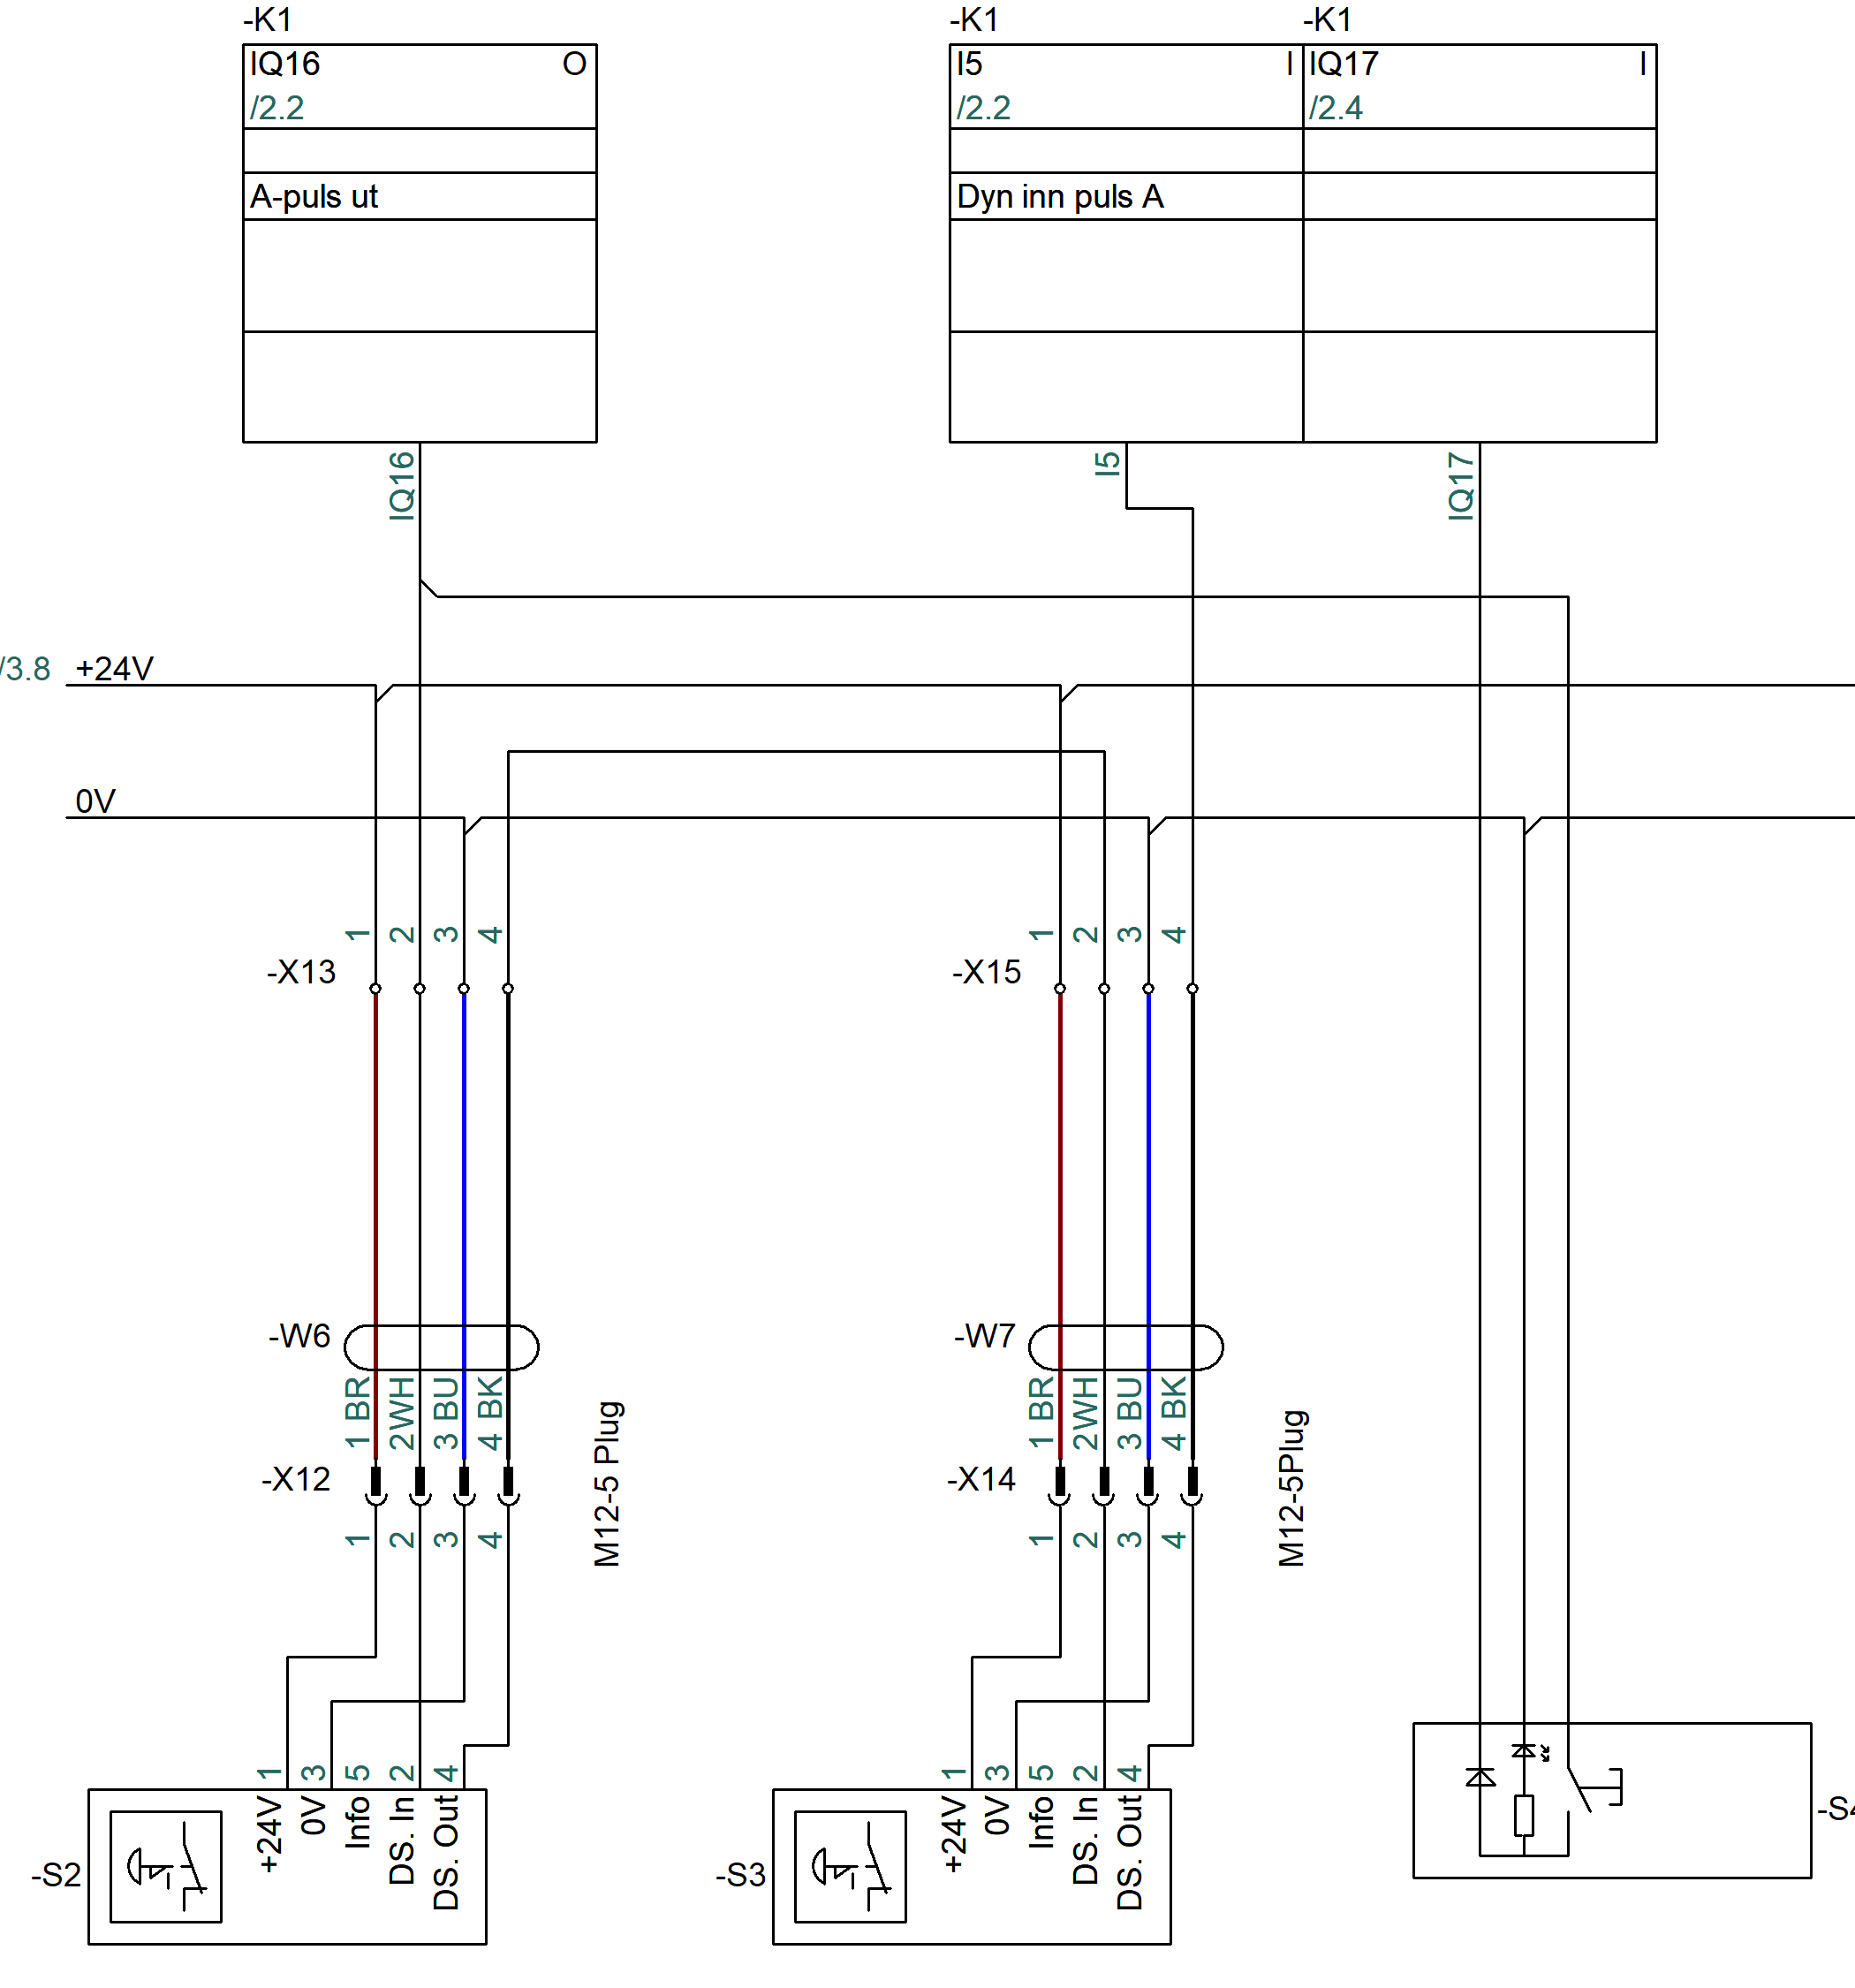
\includegraphics[width=10cm]{./aFab2324x3-4.png}$$
$$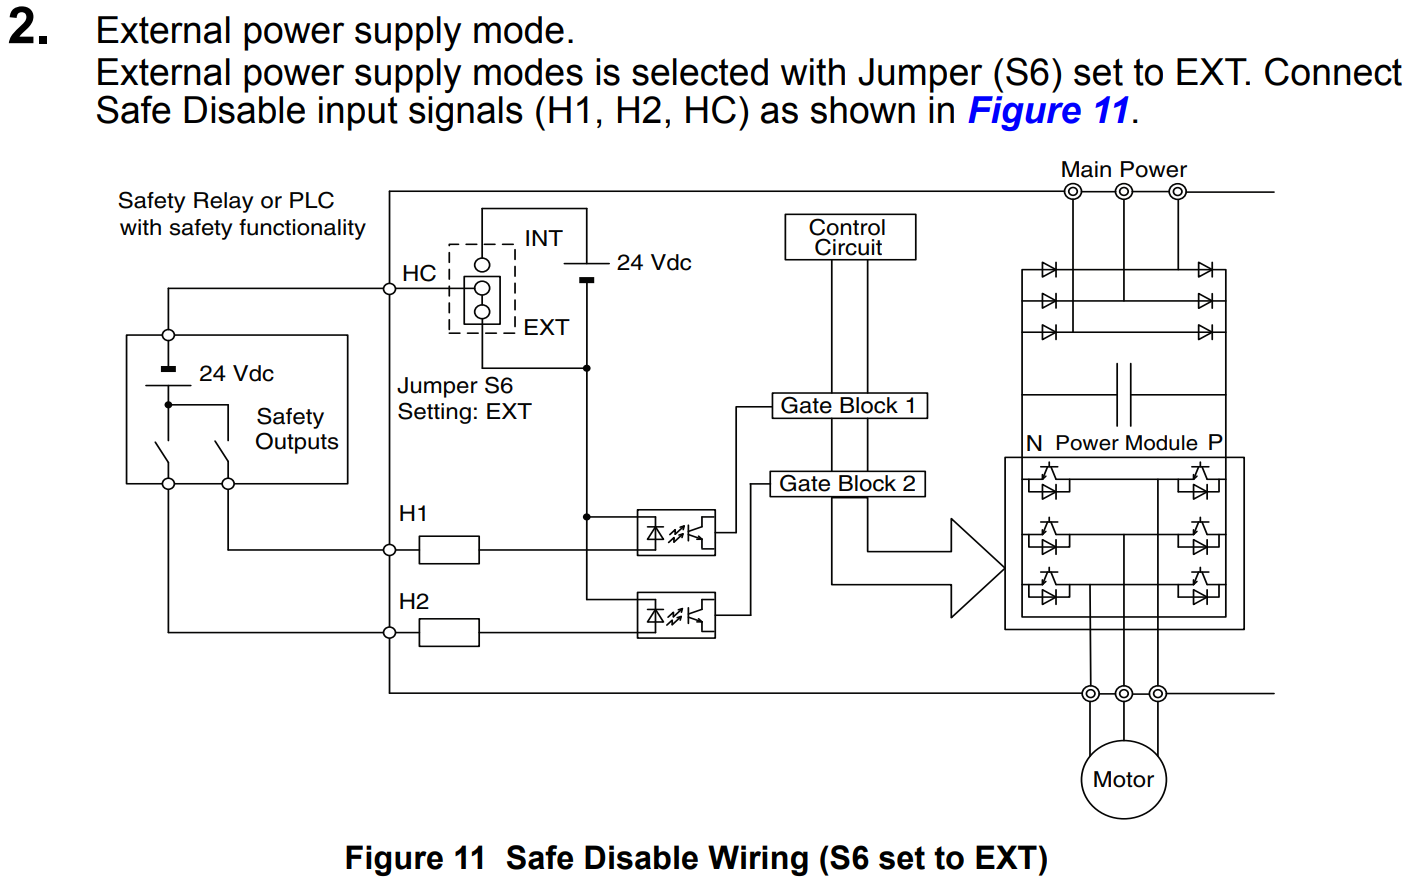
\includegraphics[width=15.5cm]{./aFab2324x3-6.png}$$
$$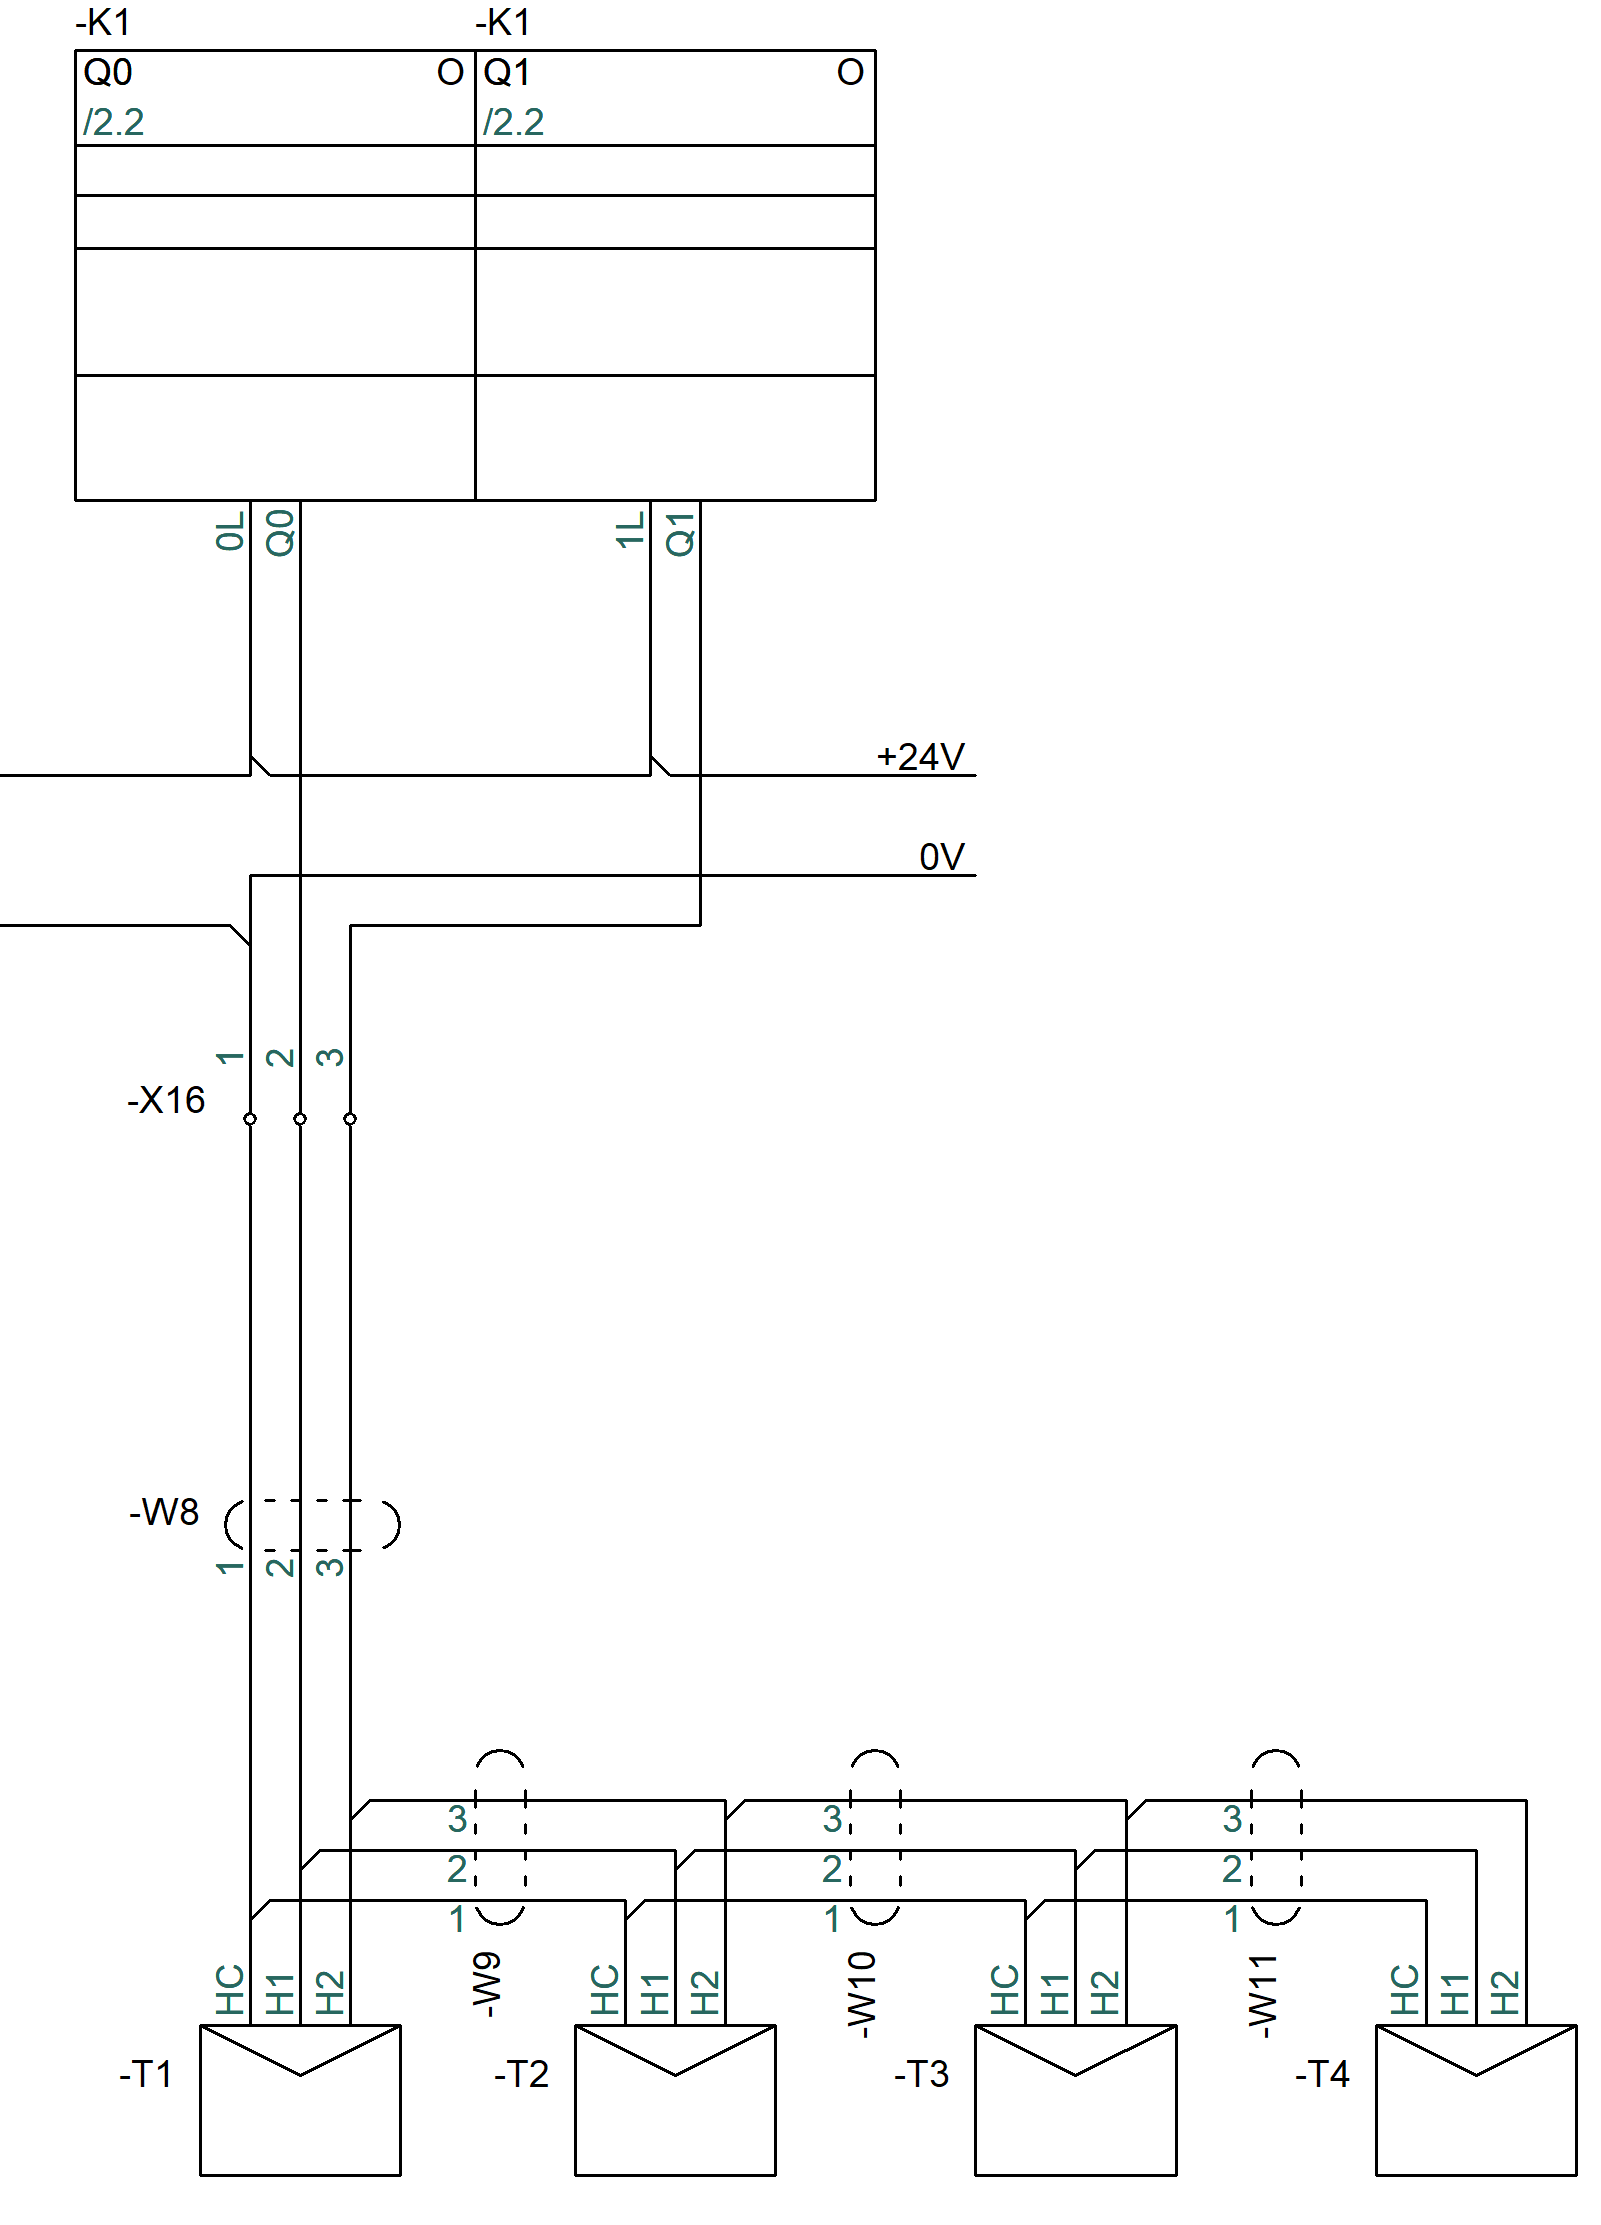
\includegraphics[width=10cm]{./aFab2324x3-7.png}$$
$$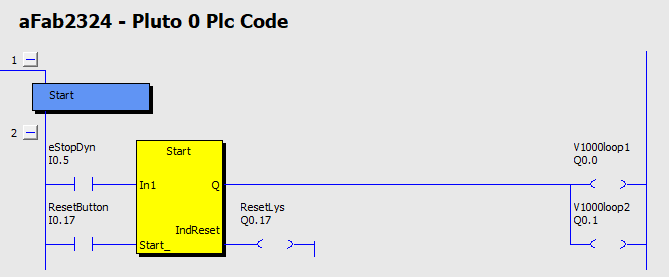
\includegraphics[width=10cm]{./aFab2324x3-8.png}$$
\oppgave{}%7
Etter at anlegget har vert i drift en stund stopper sekvensen i hjørnet mellom de to transportbåndene. Du får i oppdrag om å finne feilen. 
\vskip 1cm
• Planlegg, beskriv gjennomføring og dokumenter jobben. Lag skisser til forklaringene. 
\vskip 1cm
\oppgave{}%7
Du har fått en ny kollega og han spør om du kan forklare følgende begreper om roboten som brukes: 
\vskip 0.4cm
• Jogging 
\vskip 0.4cm
• TCP 
\vskip 0.4cm
• Workobject 
\vskip 0.4cm
• MoveL i forhold til MoveJ
\vskip 1cm
• Planlegg, beskriv gjennomføring og dokumenter jobben. Lag skisser til forklaringene. 
\vskip 1cm
\includepdf[pages=-,angle=90]{../eq/afgvformler.pdf}
\end {document}
